% !TEX root = ../main.tex
% called by main.tex
\chapter{Generalidades para el diseño}\label{ch:cad-recommendations}

\section{Puentes y geometría no soportada}
Durante el diseño de numerosas piezas, es muy frecuente encontrarse en una situación donde la geometría requiere voladizos. Estos requisitos pueden ser de origen estructural, garantizando que la orientación de las capas va a ir según los esfuerzos, estéticos, o simplemente porque la única orientación en la que la pieza se puede imprimir es con voladizos.
\par La primera recomendación a la hora de diseñar este tipo de características en una pieza \textbf{es evitarlas}. Sin embargo, por los motivos explicados anteriormente, es posible que no quede más remedio. En esos casos, se presentan a continuación algunas formas de conservar las características y asimismo mejorar la geometría para una impresión más eficiente.

\subsection*{Añadir un chaflán al voladizo}
Una de las mejores formas de facilitar la impresión de estas características es evitando el voladizo (desde el punto de vista de la impresora). Esto se puede conseguir añadiendo material de forma gradual para construir la plataforma sobre la que se irán depositando las capas del voladizo. De esta forma, se evita la necesidad de material de soporte, optimizando la impresión de las piezas. Esta geometría se puede conseguir muy fácilmente con un redondeo de los bordes o un chaflán.

\begin{figure}[ht]
	\centering
	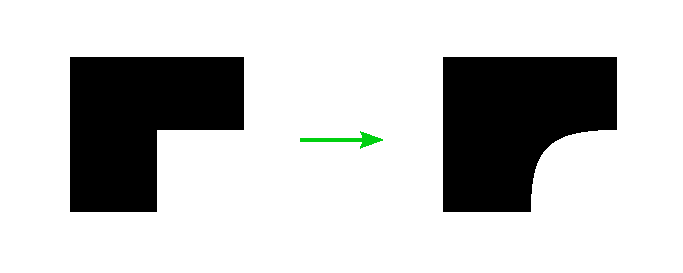
\includegraphics[width=0.6\linewidth]{figures/chaflan.pdf}
	\caption{Ejemplo de cómo un redondeo permite la impresión de un voladizo}
	\label{fig:overhang-idea}
\end{figure}

\subsection*{Soportar el voladizo en ambos extremos}
Si se busca conseguir un ``techo,'' se pueden mejorar notablemente los resultados al soportar el mismo en los dos extremos, especialmente si se aplican las sugerencias de la sección anterior y se añaden chaflanes (o \textit{fillets}). De esta forma, la distancia que será impresa sin soporte será lo menor posible, siempre que el resto de restricciones de diseño lo permitan.

\begin{figure}[ht]
	\begin{subfigure}[t]{0.49\textwidth}
		\centering
		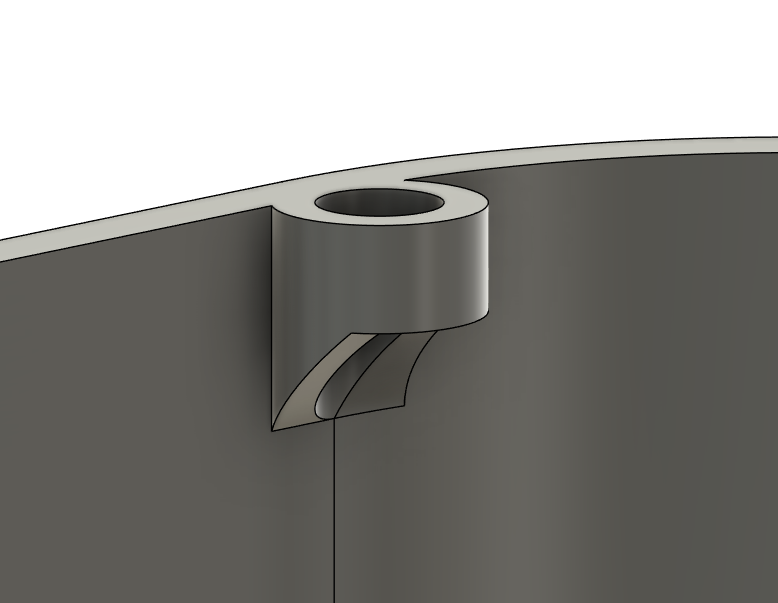
\includegraphics[width=\linewidth]{figures/chaflan.png}
		\caption{Ejemplo de un chaflán en geometría de fijación}
		\label{fig:fusion-chaflan}
	\end{subfigure}
	\hfill
	\begin{subfigure}[t]{0.49\textwidth}
		\centering
		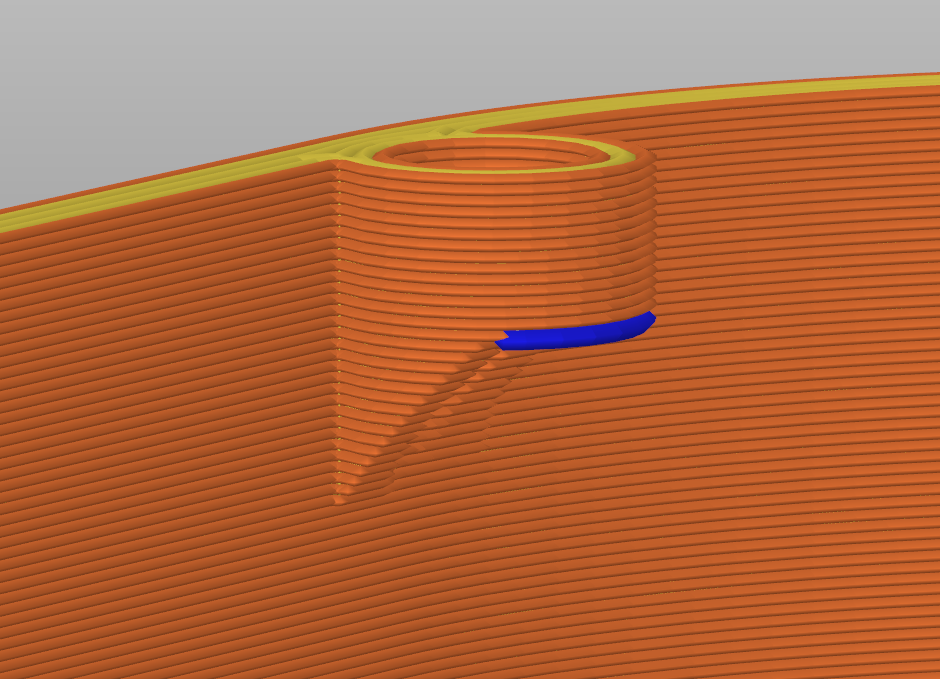
\includegraphics[width=\linewidth]{figures/chaflan-prusa.png}
		\caption[GCODE de un chaflán en un voladizo]{GCODE de un chaflán en un voladizo. En azul se puede observar donde se sigue imprimiendo sin soportes}
		\label{fig:prusa-chaflan}
	\end{subfigure}
\end{figure}

\section{Piezas o partes de piezas estructurales}
En muchas ocasiones, sobre todo en diseños mecánicos, habrá piezas de responsabilidad estructural para el correcto funcionamiento del diseño. En estos casos, es fundamental entender el recorrido de las cargas, dónde podrá haber concentraciones de esfuerzos y retocar el diseño funcional de la pieza para poder reforzar estos aspectos.

\subsection{Cargas en un plano}
Cuando el diseño permite conocer de antemano que las cargas a las que una pieza va a estar sometida estarán contenidas en un plano, (tracción-compresión, cortantes, etc.), lo más recomendable en  la mayoría de los casos es contener todos estos esfuerzos en el plano. Por ejemplo, con un engranaje muy solicitado, como el de la \autoref{fig:engranaje-cargas}
\begin{figure}[ht]
	\centering
	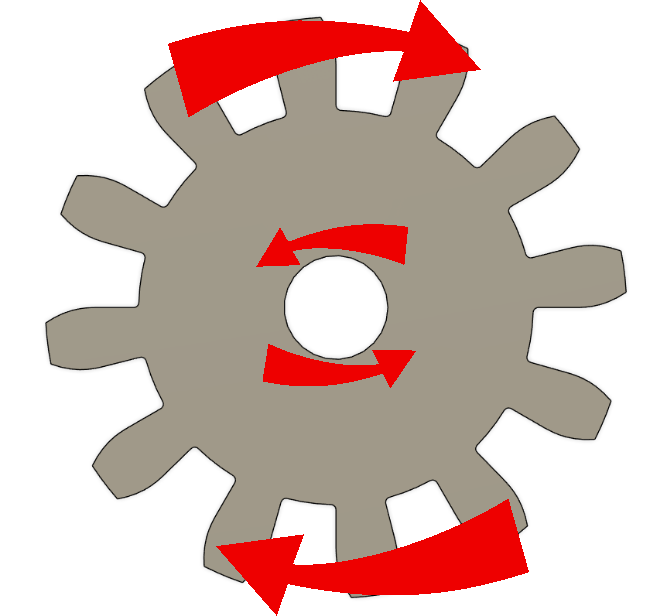
\includegraphics[width=0.5\textwidth]{figures/engranaje.png}
	\caption{Diseño de un engranaje con la previsión de las cargas}
	\label{fig:engranaje-cargas}
\end{figure}

El el caso de que sea necesario aumentar la resistencia en el plano de la pieza, una de las mejores recomendaciones es conseguir más perímetros en las direcciones de la carga. En el caso del engranaje, por contra-intuitivo que parezca, haciendo un patrón de agujeros como el de la \autoref{fig:engranaje-rediseño} puede aumentar la resistencia a fallos en el plano.
\begin{figure}[ht]
	\centering
	\begin{subfigure}[b]{0.49\textwidth}
		\centering
		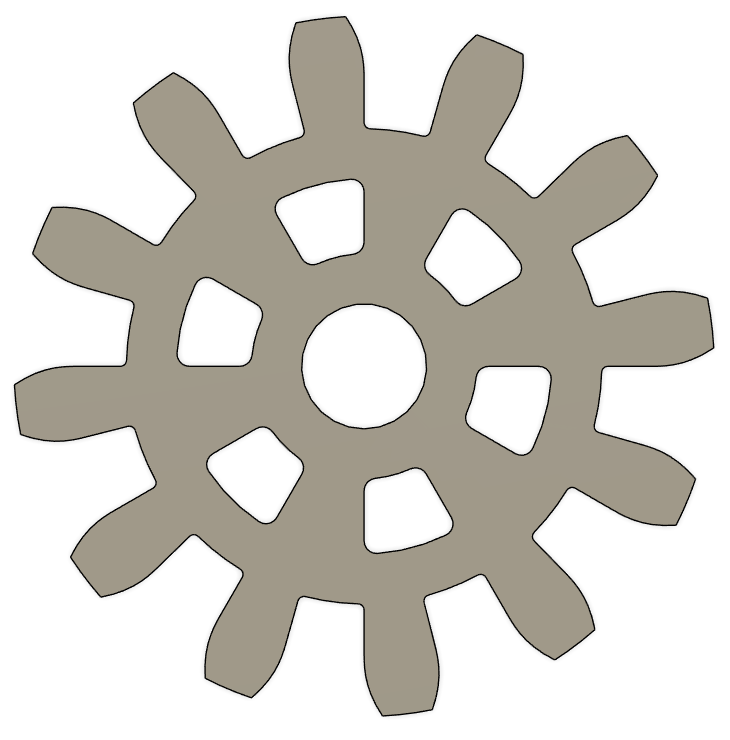
\includegraphics[width=\linewidth]{figures/engranaje-agujeros.png}
		\caption{Rediseño del engranaje para mejorar la resistencia}
		\label{fig:engranaje-agujeros}
	\end{subfigure}
	\hfill
	\begin{subfigure}[b]{0.49\textwidth}
		\centering
		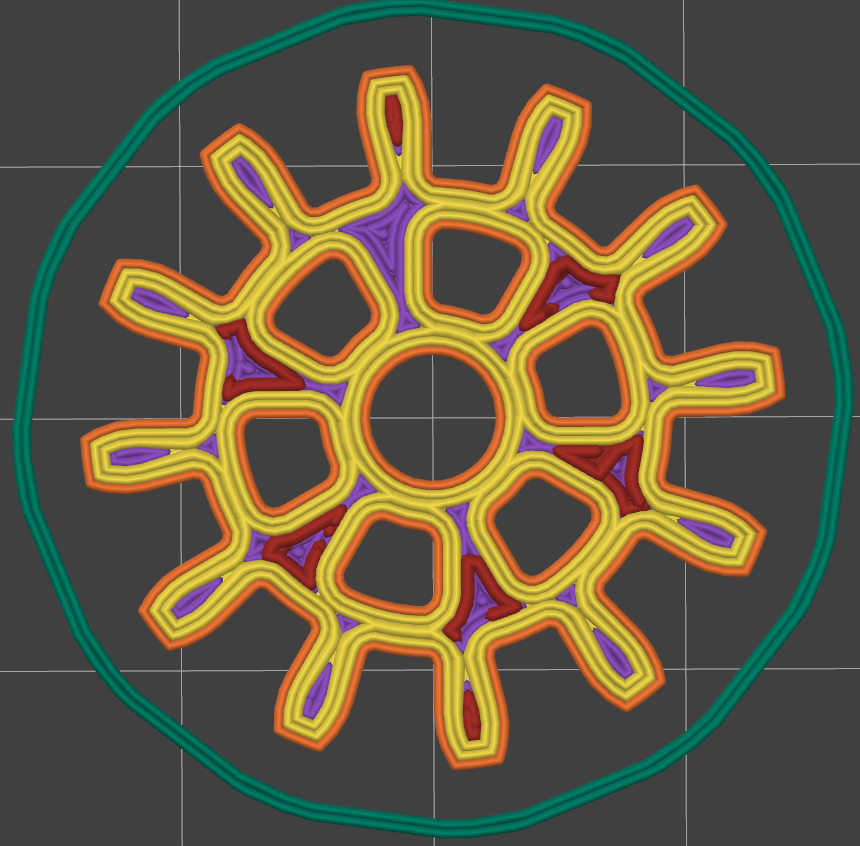
\includegraphics[width=\linewidth, angle=90]{figures/engranaje-agujeros-slice.png}
		\caption{Vista del GCODE}\label{fig:engranaje-agujeros-slice}
	\end{subfigure}
	\caption{Rediseño del engranaje}\label{fig:engranaje-rediseño}
\end{figure}

\section{Ejes y montajes con tolerancias estrechas}
Continuando con el tema de diseños mecánicos donde va a haber movimiento entre piezas, van a ser fundamentales los ``ejes'' y los montajes con tolerancias.
\par Detallar los procedimientos para diseño de este tipo de mecanismos es algo mucho más complejo de lo que esta guía pretende abarcar, incluso sin tener en cuenta que esto debe ser para piezas optimizadas para la impresión 3D. En su defecto, se proponen a continuación una serie de guías interesantes para asistir con el diseño funcional de estas piezas.

\subsection{Ejes no impresos}
En primer lugar, una de las mejores recomendaciones es considerar utilizar ejes no impresos, ya que los materiales metálicos (acero, o aluminio) en el formato de barras redondas (mecanizadas o extruidas), son baratos y accesibles, y su inclusión en los diseños puede mejorar notablemente el funcionamiento y la resistencia del producto final.
\par Sin embargo, la utilización de ejes no impresos en mecanismos de grandes solicitaciones implica otro tipo de consideraciones, entre ellas:
\begin{itemize}
	\item Correcta orientación de las capas en las piezas que interactúan con el eje
	\item Posible desgaste por fricción de las piezas que interactúan con el eje
	\item Montaje del conjunto
\end{itemize}
De todas las anteriores, probablemente la consideración más importante es la del montaje, ya que utilizar una pieza más para el eje es añadir complejidad al conjunto. Al diseñar esto, se debe asegurar que el montaje es posible, aunque se complique de forma notable.

\subsection{Montajes con tolerancias estrechas}
Para este tipo de montajes, el mejor consejo es el siguiente: evitarlos. Cuando se deben montar varias piezas con tolerancias estrechas, debido a las irregularidades de la impresión 3D, se busca que los montajes queden clasificados como montajes con `interferencia'. Esto quiere decir que dos piezas, en sus dimensiones nominales, compartirán un espacio y tiempo (lo que debería ser imposible si no hubiera deformación). Para mejorar este tipo de uniones o montajes, la recomendación es añadir mecanismos flexibles a las piezas que permitan acomodar las posibles variaciones en las dimensiones de los elementos del montaje. \todo{añadir imágenes ilustrativas de montajes `flexibles'}
\par La idea con la que el diseño se debe realizar es que si en lugar de querer montar las piezas perfectas del software CAD, se montaran algo un poco más ``amorfo'', todo vaya bien porque las piezas son flexibles \textbf{donde importa}.

\subsection{Agujeros}
Este tipo de geometría, cuando es funcional, no necesita mucha especificación. No obstante, es interesante mencionar los fallos más típicos que se pueden dar, sobre todo para la interacción entre varias piezas.
\par Los agujeros se suelen deformar cuando se imprimen en la dirección perpendicular a las capas. Una recomendación sería incluir, cuando la precisión dimensional sea necesaria, modificaciones en el propio diseño del agujero, para que este no sea exactamente circular sino que el ángulo del saliente esté limitado.

\begin{figure}[ht]
	\centering
	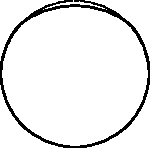
\includegraphics[width= 0.20\linewidth]{figures/agujero-rediseño.pdf}
	\caption{Muestra de cómo puede quedar un agujero habiendo aplanado la parte superior.}
	\label{fig:agujero-rediseño}
\end{figure}

\subsection{Juntas en Cola de Milano}
Este tipo de juntas son geniales para conseguir montajes rápidos e inequívocos (si se utilizan correctamente). \todo{añadir foto de junta en cola de milano, explicar cómo hacerla asimétrica.} Su principal función es la unión rígida de componentes, teniendo en cuenta que la versión más básica de esta unión no soportará cargas en una dirección (la que desmontaría la junta).

\section{Piezas planas o placas}
A la hora de imprimir piezas planas o placas, es muy importante considerar si es realmente necesario imprimirlas. En la mayoría de los casos, las piezas con esta geometría se pueden diseñar para tener unos requisitos dimensionales menos estrictos y poder ser fabricada mediante otros métodos (como en madera con taladros).
\par No obstante, puede ser interesante imprimir en 3D plantillas para la fabricación de estas piezas (un localizador para los agujeros, por ejemplo).
